%------------------------------------------------------------------------------
% Tema 8. Disfuncions del metabolisme glucídic
%------------------------------------------------------------------------------
\section{Disfuncions del metabolisme glucídic}
\label{sec:disf-del-metab}

\subsection{Regulació de la concentració de la glucosa sanguínia}
\label{sec:regulacio-de-la}
Els nivells normals de glucosa en sang són de 3,89-5,83 mmols/L
(70-105 mg/dL).

Els ajustaments constants que mantenen els nivells de glucosa en sang
prop de 4,5 mM són el resultat de l'acció combinada de la insulina,
glucagó, adrenalina i cortisol sobre els processos metabòlics que
tenen lloc en molts teixits corporals, però especialment al múscul, al
fetge i al teixit adipós. 

\begin{itemize}
\item \textbf{Insulina:} indica als teixits que els nivells de glucosa
  en sang són elevats, per sobre d'allò necessari, i per tant estimula
  la captació, la gluconeogènesi i la lipogènesi. 
\item \textbf{Glucagó:} transmet el missatge que els nivells de
  glucosa en sang són massa baixos, i els teixits responen generant glucosa per
glucogenòlisi i gluconeogènesi (fetge) i oxidant els lípids per reduir
el consum de glucosa. 
\item \textbf{Adrenalina:} s'allibera ràpidament en sang per preparar els músculs
esquelètics, pulmons i cor per un esforç sobtat i important. El
metabolisme s'ha d'adaptar ràpid, i es mobilitza més glucosa al múscul
i a l'encèfal. 
\item \textbf{Cortisol:} facilita la resposta corporal a l'estrès de llarga durada
(ansietat, por, dolor, hemorràgia, infeccions, hipoglucèmia,
inanició). Permet subministrar a l'organisme el combustible necessari
per afrontar l'estrès actuant sobre múscul, fetge i teixit adipós. És
una hormona d'acció lenta que modifica el nivell d'expressió enzimàtic
en les cèl·lules diana.
\end{itemize}

\begin{figure}[H]
  \centering
  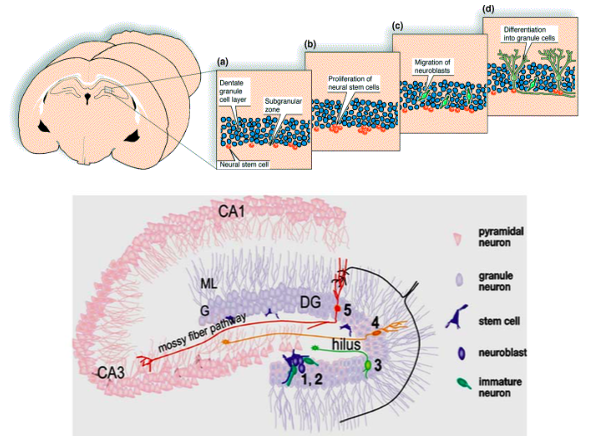
\includegraphics[width=1\textwidth]{fig27}
  \caption{Mecanismes hormonals de regulació de la homeòstasi de
    glucosa}
  \label{fig:fig27}
\end{figure}

\subsection{Hiperglucèmies}
\label{sec:hiperglucemies}
Hi ha 4 tipus d'hiperglucèmia:
\begin{itemize}
\item \textbf{Diabetis tipus 1:} Hiperglucèmia de manera abrupta. Els pacients
  necessiten insulina per sobreviure.
\item \textbf{Diabetis tipus 2:} Progressió gradual i la insulina no acostuma a
  ser necessària pel tractament.
\item \textbf{Altres tipus específics}
\item \textbf{Diabetis gestacional:} Es produeix en l'últim terç de la
  gestació. Normalment acaba després del part però en alguns casos el
  quadre hiperglucèmic continua.
\end{itemize}

Hi ha 2 subgrups poblacionals en risc de diabetis:
\begin{itemize}
\item Intolerància a la glucosa: 2h després de la ingesta de 75 de
  glucosa, els nivells de glucosa es troben entre 140 i 199 mg/dL.

\item Disfunció de la glucosa en dejuni: La glucosa es troba entre 100
  i 125 mg/dL.
\end{itemize}

Hi ha un marcador circulant usat per monitoritzar els diabètics que és
la hemoglobina $A_{1c}$. L'hemoglobina incorpora glucosa
espontàniament a la seva estructura i són un reflex dels nivells
circulants de glucosa. Aquesta hemoglobina té una vida mitja llarga.

Els nous criteris diagnòstics de la diabetis són:
\begin{itemize}
\item Símptomes de diabetis més una concentració casual (no en dejuni)
  de glucosa superior a 200 mg/dL.
\item Glucosa en plasma després d'un dejuni mínim de 8 hores superiors
  a 126 mg/dL.
\item Glucèmia superior a 200 mg/dL després de 2 hores del test de
  tolerància oral de glucosa.
\item Nivells Hb$A_{1c}$ superiors a 6,5\%.
\end{itemize}

\begin{table}[H]
  \centering
\begin{tabular}{ccc>{\centering}p{3cm}}
\cline{3-4} 
 &  & \textbf{\textsc{Tipus 1}} & \textbf{\textsc{Tipus 2}}\tabularnewline
\hline 
\textbf{Edat habitual} &  & < 30 & > 35\tabularnewline
\hline 
\textbf{Símptomes} &  & Poliúria & Assimptomàtica\tabularnewline
 &  & Polidípsia & \tabularnewline
 &  & Polifàgia & \tabularnewline
\hline 
\textbf{Aspecte físic} &  & Consunció & Obesitat\tabularnewline
 &  & Deshidratació & \tabularnewline
 &  & Pèrdua de consciència & \tabularnewline
\hline 
\textbf{Cetoacidosi} &  & Molt freqüent & Absent\tabularnewline
\hline 
\textbf{Resposta a insulina} &  & Sensible & Resistent\tabularnewline
\hline 
\textbf{Tractament} & Dieta & Insuficient & Suficient\tabularnewline
 & Insulina & Essencial (ràpida+lenta) & A vegades\tabularnewline
 & Altres & ----- & Metformina, sulfonilurees\tabularnewline
\hline 
\textbf{Origen} & Herència poligènica & Al·lels MHC-I & Múltiples alteracions\tabularnewline
 & Factors ambientals & Virus & Dietes grasses, obesitat, edat\tabularnewline
\hline 
\end{tabular}
  \caption{Tipus de diabetis més freqüents}
  \label{tab:tab_diabetis}
\end{table}

\subsubsection{Alteracions metabòliques}
\label{sec:alter-metab}
Les més importants són:
\begin{itemize}
\item Els individus amb qualsevol dels dos tipus de diabetis són
  incapaços de captar eficientment la glucosa de la sang, ja que la
  insulina provoca el desplaçament dels transportadors de glucosa
  GLUT4 a la membrana plasmàtica del múscul i del teixit adipós. La
  glucosa no pot rebaixar els seus nivells.

\item La manca de captació d’insulina o la manca d’insulina circulant
provoca que les cèl·lules només responguin al glucagó. Fins i tot, en
el cas que les cèl·lules $\beta$ dels illots de Langerhans hagin
desaparegut, les cèl·lules α poden proliferar més d’allò normal. Els
efectes del glucagó sobre el fetge provoquen, per exemple, un
increment de la GNG (amb consum d’intermediaris del cicle de Krebs) i
de la glucogenòlisi, de tal manera que s’allibera més glucosa en
sang. 


\item A nivell muscular, s’estimula la degradació proteica per abastir
  el fetge de substrats gluconeogènics.

\item L’acumulació de glucosa en sang (també afavorida per
  l’alliberament d’AG, que bloqueja la captació de glucosa), suposa
  que el ronyó comenci a excretar glucosa en l’orina (glucosúria). Com
  que es força el ronyó, una situació d’aquest tipus perllongada pot
  conduir a una insuficiència renal.

\item Com que falta glucosa, els AG es converteixen en el combustible
  principal, fet que porta a un altre canvi metabòlic característic:
  l’oxidació excessiva però incompleta dels AG al fetge. L’acetil-CoA
  produït en la $\beta$-oxidació no pot ser oxidat completament pel cicle de
  Krebs, ja que l’elevada proporció [NADH]/[NAD] produïda per la
  $\beta$-oxidació inhibeix el cicle (hi ha 3 passos del cicle que
  converteixen NAD en NADH).

\item L’acumulació d’acetil-CoA, juntament amb l’estímul de la GNG,
  ocasiona una sobreproducció dels cossos cetònics acetoacetat i
  $\beta$-hidroxibutirat, que no poden ser usats pels teixits al
  mateix ritme que els sintetitza el fetge. 

\item A més, l’acetoacetat pot patir una descarboxilació espontània i
  esdevenir acetona. L’acetona en nivells alts és detectable per l’alè
  afruitat (és volàtil, de vegades es confon amb l’etanol) i en
  l’orina.

\item La sobreproducció de cossos cetònics (cetosi) es manifesta per
  un augment de la seva concentració en sang (cetonèmia) i en orina
  (cetonúria). Com que els cossos cetònics són àcids carboxílics que
  s’ionitzen alliberant protons, en la diabetis no controlada aquesta
  producció d’àcids pot sobrepassar la capacitat amortidora del
  sistema de bicarbonat de la sang i produir una acidosi, denominada
  cetoacidosi, que és un risc per a la vida de l’individu. Per
  exemple, pot produir un coma diabètic. 
\end{itemize}

\subsubsection{Complicacions}
\label{sec:complicacions}
Alteracions de la microvasculatura i la macrovasculatura. Els vasos es
malmeten i generen gangrena sobretot als peus.

Hi ha neuropatia. També hi pot haver retinopatia diabètica.

Els ronyons també pateixen un dany. La glucosa és un osmòlit, i com
que la concentració és tant alta no es pot reabsorbir a nivell
tubular. La glucosa malmet els glomèruls renals. L'epiteli fenestrat
presenta càrregues negatives i impedeix el pas de proteïnes. La
glucosa alta fa que els glomèruls siguin més permeables i que a la
orina hi hagi més proteïnes, majoritàriament albúmina perquè és la
proteïna més abundant del plasma i té un pes de 65 kDa, límit de mida
per filtrar als glomèruls (60 kDa).

També hi ha més risc de patir aterosclerosi. Sembla que estar
relacionada amb un procés de glicosilació de la superfície de les
lipoproteïnes.

\subsection{Paràmetres clínics}
\label{sec:parametres-clinics}

\subsubsection{Glucosa}
\label{sec:glucosa}
El \textbf{mètode de l'ortotoluïdina} consisteix que en medi àcid, la glucosa
reacciona amb amines aromàtiques i genera color. Un altre mètode, el
de Benedict està basat en la reducció del Cu (usat en tires reactives
per la orina).

El mètode de referència és el mètode que han de tenir tots els
laboratoris i poder avaluar la qualitat inter-laboratoris. Per la
glucosa, és el \textbf{mètode basat en la hexoquinasa} i la
glucosa-6-P-deshidrogenasa. La reacció genera NADPH, que es pot
mesurar a 340 nm.

Hi pot haver diferents fonts de variabilitat pre-metrològica:
\begin{itemize}
\item Sang/Sèrum o plasma. Normalment no s'usa sang total, ja que els
  eritròcits consumeixen glucosa i els valors sortirien més baixos
  dels reals.
\item La concentració arterial és superior a la venosa.
\item L'edat, els fàrmacs (corticoides i diürètics) augmenten la
  glucosa.
\end{itemize}

S'han de prendre diferents precaucions:
\begin{itemize}
\item No ha de ser sang total (eritròcits contenen < [glc])
\item Cal ser ràpids per evitar metabolisme eritrocitari
\item Desproteinització prèvia per evitar interferències
\item Estabilitat 8h a 25ºC - 72h a 4ºC
\end{itemize}

\subsubsection{Sobrecàrrega oral de glucosa (SOG)}
\label{sec:sobrecarrega-oral-de}
Si surt un valor alt de glucèmia, es repeteix l'analítica. Si torna a
sortir hiperglucèmia es practica un test de sobrecàrrega oral de
glucosa o test de tolerància oral a la glucosa. Aquest test es
realitza en 4 situacions:
\begin{enumerate}
\item Diabetis gestacional
\item Intolerància a la glucosa (IGT)
\item Neuropaties, nefropaties o retinopaties. En casos que la
  glucèmia sigui inferior a 140 mg/dL (7,7 mM).
\item Estudis epidemiològics
\end{enumerate}

El test consisteix en ingerir 75g de glucosa pels adults i 1,75 g de
glucosa/kg en nadons i nens. S'extreu sang a $t_0$ en dejuni i en
situació normal. Cada cert temps es mesura la glucèmia i s'avalua
l'evolució de la glucèmia. Els resultats poden ser:
\begin{enumerate}
\item Normal: Pic abrupte a 30 minuts fins que a les 2h es normalitza
  la glucèmia.
\item Diabetis: Fa un pic abrupte a 30 min i després un  plateau més o
  menys estable.
\item Intolerant: Perfil intermig.
\end{enumerate}

En el cas de la diabetis gestacional, es fa un \textit{screening} cap
a les 24 setmanes de gestació. El test de O'Sullivan no requereix que
la gestant estigui en dejuni. S'administren 50 g de glucosa i es
mesura la glucèmia al cap d'1h. Si surt la glucèmia superior a 7,7 mM
es practica un test de SOG però amb 100 g de glucosa i es mira si la
glucosa al cap de 2h és inferior a 9,4 mM o bé si hi ha 2 punts de la
corba per sobre del llindar.

\subsubsection{Insulina}
\label{sec:insulina}
En el SOG, en paral·lel a la glucosa es pot determinar la insulina. No
es fa normalment. En situació normal, el perfil d'insulina és
paral·lel al de la glucosa. 

\begin{figure}[H]
  \centering
  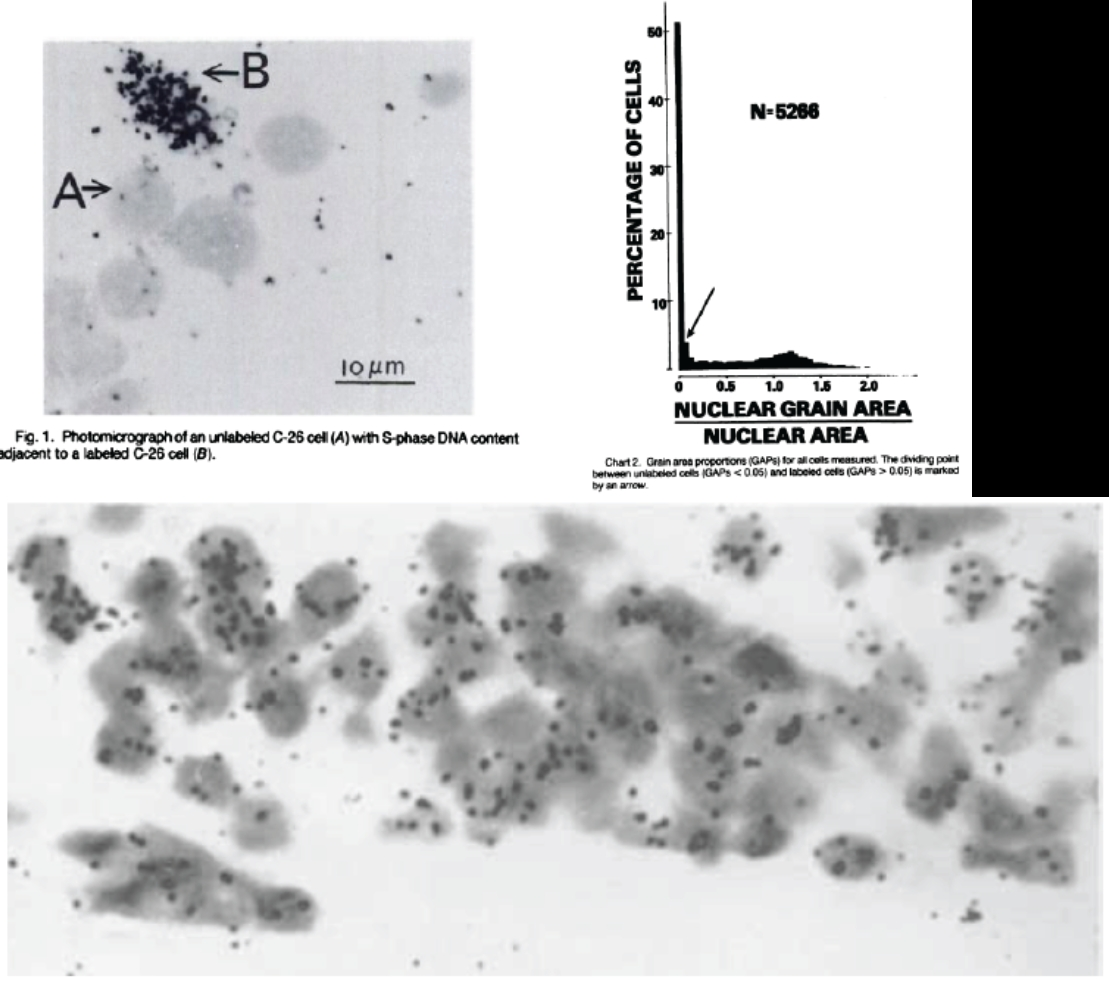
\includegraphics[width=0.85\textwidth]{fig28}
  \caption{Perfil de secreció d'insulina}
  \label{fig:fig28}
\end{figure}

Hi ha diferents situacions on és interessant determinar la insulina:
\begin{enumerate}
\item Hipoglucèmia
\item Insulinoma (tumor que secreta insulina)
\item Diabètic amb sobredosi
\end{enumerate}

La insulina presenta nivells molt baixos en sang (20 mU/L, < 118 pM) i
es determina per RIA. Durant el SOG, els valors inferiors a 430 pM a
t120 descarten la resistència a insulina.

El pèptid C és resultat de la proteòlisi de la pro-insulina. La vida
mitja del pèptid C circulant és més alta que la de la insulina. Al
fetge s'elimina el 75\% de la insulina circulant. La relació pèptid
C/insulina és equimolar. Normalment, hi ha 5-10 vegades més pèptid C
que insulina. Els nivells normals de pèptid C són de 1-2 ng/mL i es
determina per RIA.
\begin{enumerate}
\item Si hi ha nivells elevats d'insulina i pèptid C, és símptoma
  d'insulinoma.
\item Si hi ha més insulina que pèptid C, vol dir que hi hagut una
  intoxicació per insulina.
\end{enumerate}

\subsubsection{Glicohemoglobines}
\label{sec:glicohemoglobines}


\subsubsection{Fructosamines}
\label{sec:fructosamines}


\subsubsection{Cossos cetònics}
\label{sec:cossos-cetonics}


\subsection{Hipoglucèmies}
\label{sec:hipoglucemies}

\subsubsection{Fisiològica}
\label{sec:fisiologica}
En diferents situacions metabòliques com:
\begin{itemize}
\item Post-pandrial: 1-3 hores després d'un àpat
\item Post-absortiva: 6-10 hores després de l'últim àpat. Sol ser
  nocturna.
\item Cetòtica
\end{itemize}

\subsubsection{Patològiques}
\label{sec:patologiques}
N'hi ha de diferents tipus:
\begin{itemize}
\item Congènita
\item Eritroblastosi: Hiperplàsia pancreàtica
\item Glicogenosi: Es poden dividir segons el teixit afectat
  \begin{itemize}
  \item Hepàtic: La síndrome de Von Gierke o de tipus I està causat per una
    deficiència de glucosa-6-fosfatasa (GNG i glicogenòlisi). En
    dejuni, el fetge no pot corregir la hipoglucèmia.

  \item Muscular o miopàtic: Deficiència en glicogen fosforilasa muscular. És la
    malaltia de McArdle o de tipus V. Es manifesta quan es fa exercici
    físic.

  \item Generalitzada: La malaltia de Pompe és una glicosidasa
    lisosomal. Els individus no mobilitzen bé el glicogen en molts
    teixits.

La glicogenosi de tipus III o de Cori-Forbes és l'enzim
desramificador. L'enzim desramificador produeix glucosa lliure. Té un
fenotip lleu.

\item Alteracions del metabolisme de la fructosa: Fructosúria
  essencial. Provocada per un dèficit de fructoquinasa al fetge. Es
  pot fosforilar per hexoquinasa, a molt baixa velocitat.

La intolerància hereditària a la fructosa està provocada per una
deficiència en aldolasa B (hidrolitza fructosa-1-fosfat). S'ha
d'evitar la fructosa a la dieta. Generen hipoglucèmia, hepatomegàlia,
icterícia.

El dèficit en fructosa-1,6-difosfat provoca una deficiència de GNG
hepàtica i hipoglucèmia.  

\item Alteracions del metabolisme de la galactosa: S'ha d'evitar la
  ingesta de lactosa. Els malalts desenvolupan cataractes degut a
  l'acumulació de galactitol al cristal·lí.
  \end{itemize}
\end{itemize}

També poden ser deguts a xenobiòtics (fàrmacs), alcoholisme,
insulinoma o hipoglucèmia reactiva (hipereficiència del pàncrees).

\subsection{Intoleràncies}
\label{sec:intolerancies}
La més prevalent és la intolerància a la lactosa degut a la
deficiència de lactasa intestinal. L'expressió adulta de la lactasa
depèn de la dieta.